Following \cite{VanTrees2002DetectionIV}'s half power beam width (HPBW) calculation steps assuming classic passive ULA under the conventional beamformer, we start at equation (2.96) which express the beampattern in $u$-space, stating that
$$
B_{u}\left(u\right)=
\frac{1}{N}
\frac{
sin\left(\frac{\pi{}Nd}{\lambda}u\right)
}{
sin\left(\frac{\pi{}d}{\lambda}u\right)
}.
$$
In this paper, we define $\dTheta = \frac{2\pi{}d\left(\cos\left(\theta_{g}\right)-\cos\left(\theta_{g,s}\right)\right)}{\lambda}$, therefore
$$
B_{\theta_{g}}\left(\theta_{g}\right)=
\frac{1}{N}
\frac{
\sin\left(N\dTheta\right)
}{
\sin\left(\dTheta\right)
},
$$
i.e.
\begin{equation}
     u = 2\cos\left(\theta_{g}\right).
\end{equation}
Comparing $B_{u}\left(u\right)$ to $1/\sqrt{2}$ for the extraction of $u_{HPBW}$, \cite{VanTrees2002DetectionIV} determines (equation 2.98) that the HPBW is achieved by setting 
\begin{equation}
    \label{eqn_classicULA_beamwidthCalc_VanTrees_eq_2_98}
    \frac{\pi{}Nd}{\lambda}u = 1.4
\end{equation}
and hints in the matching problem (2.4.7) that the number $1.4$ can be calculated using the $2^{nd}$ order taylor expansion of $B_{u}\left(u\right)$. Equivalent analysis of $ f_{N}\left(x\right)\triangleq\frac{\sin\left(Nx\right)}{\sin\left(x\right)} $ and expansion to its second order terms (i.e.
$
\evalat{f\left(x\right)}{x\to{}a,} \approx 
f(a) + 
\frac{1}{1!}\evalat{\frac{\partial{f}}{\partial{x}}}{\left(x=a\right)}\left(x-a\right) 
+ 
\frac{1}{2!}\evalat{\frac{\partial{f}}{\partial{x^{2}}}}{\left(x=a\right)}\left(x-a\right)^{2}
$), results in
\begin{equation}
    \evalat{f\left(x\right)}{x\to0}
    \approx
    1 + \frac{1}{2!}\left(\frac{1-N^{2}}{3}\right)x^{2}.
\end{equation}
Comparing to $1/\sqrt{2}$, one can write
\begin{equation*}
    Nx_{HPBW} = N\sqrt{\frac{6\left(1-1/\sqrt{2}\right)}{N^{2}-1}}
    \overset{N>>1}{\to} \sqrt{6\left(1-1/\sqrt{2}\right)} \approx 1.325,
\end{equation*}
which doesn't quite fit the stated value (\ref{eqn_classicULA_beamwidthCalc_VanTrees_eq_2_98}). This lead us to investigate a higher order taylor expansions. As can be verified, $\evalat{\frac{\partial{f}}{\partial{x}^{3}}}{x=0} = 0$, leading to expressing the $4^{th}$ order term
\begin{equation}
    \evalat{f\left(x\right)}{x\to0}
    \approx
    1 
    + 
    \frac{1}{2!}\left(\frac{1-N^{2}}{3}\right)x^{2}
    +
    \frac{1}{4!}\left(\frac{N^{4}}{5}-\frac{2N^{2}}{3}+\frac{7}{15}\right)x^{4}
\end{equation}
which conveniently generates a quadratic equation with respect to $x^{2}$. We plot $Nx_{HPBW}$ for various values of $N$ in fig.(\ref{fig_classicULA_beamwidth_Nx_HPBW}) and one can see that indeed, as stated in \cite{VanTrees2002DetectionIV}, $Nx_{HPBW}$ tends toward $1.4$ as $N$ increases.
\begin{figure}
    \label{fig_classicULA_beamwidth_Nx_HPBW}
    \centering
    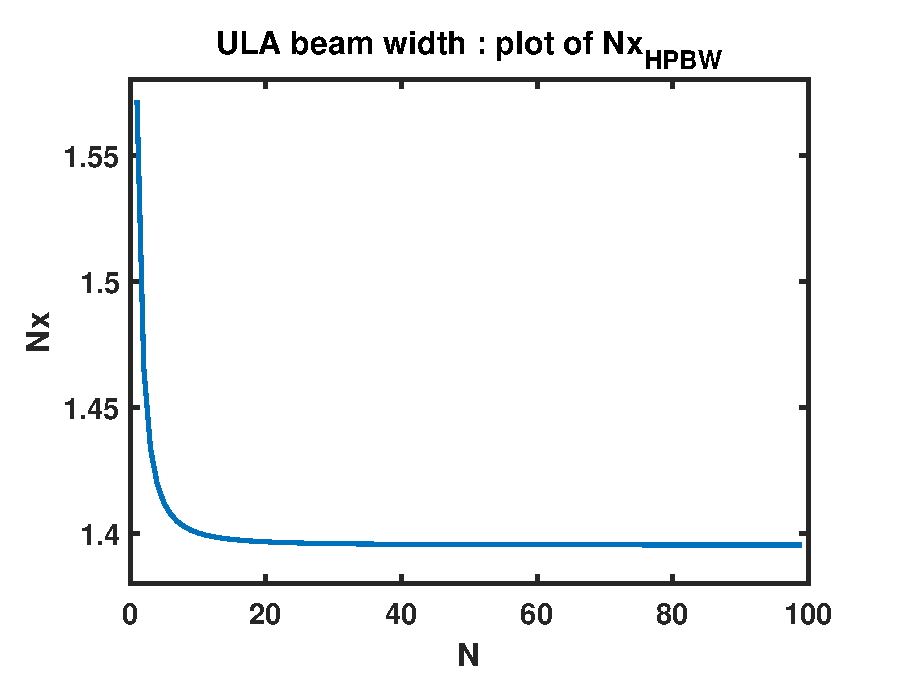
\includegraphics[width=0.6\linewidth]{./Media/spatial_IIR_MATLAB/beamwidth/Nx_HPBW.eps}
    \caption{Plot of $Nx_{HPBW}$ for various $N$ values. For each $N$, $x_{HPBW}$ was calculated as a solution to the quadratic equation (with respect to $x^{2}$) and mutiplied by the matching $N$. Although $x_{HPBW}$ monotonically decreasing as $N$ increases, it is evident that $Nx_{HPBW}$ tends towards a finite limit of $\sim1.4$.}
\end{figure}
With \cite{VanTrees2002DetectionIV}'s equation (2.96) (\ref{eqn_classicULA_beamwidthCalc_VanTrees_eq_2_98} in our paper) proven, using the fact that $u = 2\cos{\theta_{g}}$ (where $\theta_{g}$ is the geometric angle), one can write that
$$
u_{HPBW} = \frac{\lambda}{Nd}\frac{1.4}{\pi}.
$$
Therefore, considering that $B_{u}\left(u\right)$ is an even function, the actual beamwidth is twice the size of $u_{HPBW}$ 
\begin{equation}
    HPBW_{u} = 2u_{HPBW} = \frac{2.8}{\pi}\frac{\lambda}{Nd} \approx 0.891\frac{\lambda}{Nd}
\end{equation}
as stated in \cite{VanTrees2002DetectionIV}'s equation (2.100). For other spaces representation of the HPBW, see \cite{VanTrees2002DetectionIV}'s (table 2.2), where for the $\theta_{g}$-space, $\Tilde{\theta_{g}} \triangleq \pi/2-\theta_{g}$ was defined to emphasize that the entire analysis of the beampattern was under the assumption that $\theta_{g,s}=\pi/2$, stating that
\begin{equation}
    \Tilde{\theta}_{g,HPBW} = 2\sin^{-1}\left(0.446\frac{\lambda}{Nd}\right)
\end{equation}
and for small $\Tilde{\theta}_{g}$ (i.e large $N$ values),
\begin{equation}
    \Tilde{\theta}_{g,HPBW} \approx 0.891\frac{\lambda}{Nd}
\end{equation}